\documentclass[1p]{elsarticle_modified}
%\bibliographystyle{elsarticle-num}

%\usepackage[colorlinks]{hyperref}
%\usepackage{abbrmath_seonhwa} %\Abb, \Ascr, \Acal ,\Abf, \Afrak
\usepackage{amsfonts}
\usepackage{amssymb}
\usepackage{amsmath}
\usepackage{amsthm}
\usepackage{scalefnt}
\usepackage{amsbsy}
\usepackage{kotex}
\usepackage{caption}
\usepackage{subfig}
\usepackage{color}
\usepackage{graphicx}
\usepackage{xcolor} %% white, black, red, green, blue, cyan, magenta, yellow
\usepackage{float}
\usepackage{setspace}
\usepackage{hyperref}

\usepackage{tikz}
\usetikzlibrary{arrows}

\usepackage{multirow}
\usepackage{array} % fixed length table
\usepackage{hhline}

%%%%%%%%%%%%%%%%%%%%%
\makeatletter
\renewcommand*\env@matrix[1][\arraystretch]{%
	\edef\arraystretch{#1}%
	\hskip -\arraycolsep
	\let\@ifnextchar\new@ifnextchar
	\array{*\c@MaxMatrixCols c}}
\makeatother %https://tex.stackexchange.com/questions/14071/how-can-i-increase-the-line-spacing-in-a-matrix
%%%%%%%%%%%%%%%

\usepackage[normalem]{ulem}

\newcommand{\msout}[1]{\ifmmode\text{\sout{\ensuremath{#1}}}\else\sout{#1}\fi}
%SOURCE: \msout is \stkout macro in https://tex.stackexchange.com/questions/20609/strikeout-in-math-mode

\newcommand{\cancel}[1]{
	\ifmmode
	{\color{red}\msout{#1}}
	\else
	{\color{red}\sout{#1}}
	\fi
}

\newcommand{\add}[1]{
	{\color{blue}\uwave{#1}}
}

\newcommand{\replace}[2]{
	\ifmmode
	{\color{red}\msout{#1}}{\color{blue}\uwave{#2}}
	\else
	{\color{red}\sout{#1}}{\color{blue}\uwave{#2}}
	\fi
}

\newcommand{\Sol}{\mathcal{S}} %segment
\newcommand{\D}{D} %diagram
\newcommand{\A}{\mathcal{A}} %arc


%%%%%%%%%%%%%%%%%%%%%%%%%%%%%5 test

\def\sl{\operatorname{\textup{SL}}(2,\Cbb)}
\def\psl{\operatorname{\textup{PSL}}(2,\Cbb)}
\def\quan{\mkern 1mu \triangleright \mkern 1mu}

\theoremstyle{definition}
\newtheorem{thm}{Theorem}[section]
\newtheorem{prop}[thm]{Proposition}
\newtheorem{lem}[thm]{Lemma}
\newtheorem{ques}[thm]{Question}
\newtheorem{cor}[thm]{Corollary}
\newtheorem{defn}[thm]{Definition}
\newtheorem{exam}[thm]{Example}
\newtheorem{rmk}[thm]{Remark}
\newtheorem{alg}[thm]{Algorithm}

\newcommand{\I}{\sqrt{-1}}
\begin{document}

%\begin{frontmatter}
%
%\title{Boundary parabolic representations of knots up to 8 crossings}
%
%%% Group authors per affiliation:
%\author{Yunhi Cho} 
%\address{Department of Mathematics, University of Seoul, Seoul, Korea}
%\ead{yhcho@uos.ac.kr}
%
%
%\author{Seonhwa Kim} %\fnref{s_kim}}
%\address{Center for Geometry and Physics, Institute for Basic Science, Pohang, 37673, Korea}
%\ead{ryeona17@ibs.re.kr}
%
%\author{Hyuk Kim}
%\address{Department of Mathematical Sciences, Seoul National University, Seoul 08826, Korea}
%\ead{hyukkim@snu.ac.kr}
%
%\author{Seokbeom Yoon}
%\address{Department of Mathematical Sciences, Seoul National University, Seoul, 08826,  Korea}
%\ead{sbyoon15@snu.ac.kr}
%
%\begin{abstract}
%We find all boundary parabolic representation of knots up to 8 crossings.
%
%\end{abstract}
%\begin{keyword}
%    \MSC[2010] 57M25 
%\end{keyword}
%
%\end{frontmatter}

%\linenumbers
%\tableofcontents
%
\newcommand\colored[1]{\textcolor{white}{\rule[-0.35ex]{0.8em}{1.4ex}}\kern-0.8em\color{red} #1}%
%\newcommand\colored[1]{\textcolor{white}{ #1}\kern-2.17ex	\textcolor{white}{ #1}\kern-1.81ex	\textcolor{white}{ #1}\kern-2.15ex\color{red}#1	}

{\Large $\underline{11a_{347}~(K11a_{347})}$}

\setlength{\tabcolsep}{10pt}
\renewcommand{\arraystretch}{1.6}
\vspace{1cm}\begin{tabular}{m{100pt}>{\centering\arraybackslash}m{274pt}}
\multirow{5}{120pt}{
	\centering
	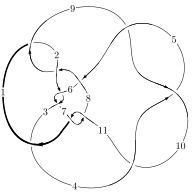
\includegraphics[width=112pt]{../../../GIT/diagram.site/Diagrams/png/596_11a_347.png}\\
\ \ \ A knot diagram\footnotemark}&
\allowdisplaybreaks
\textbf{Linearized knot diagam} \\
\cline{2-2}
 &
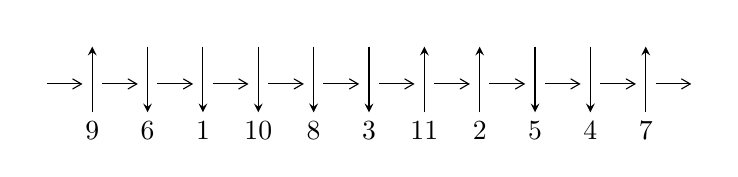
\begin{tikzpicture}[x=20pt, y=17pt]
	% nodes
	\node (C0) at (0, 0) {};
	\node (C1) at (1, 0) {};
	\node (C1U) at (1, +1) {};
	\node (C1D) at (1, -1) {9};

	\node (C2) at (2, 0) {};
	\node (C2U) at (2, +1) {};
	\node (C2D) at (2, -1) {6};

	\node (C3) at (3, 0) {};
	\node (C3U) at (3, +1) {};
	\node (C3D) at (3, -1) {1};

	\node (C4) at (4, 0) {};
	\node (C4U) at (4, +1) {};
	\node (C4D) at (4, -1) {10};

	\node (C5) at (5, 0) {};
	\node (C5U) at (5, +1) {};
	\node (C5D) at (5, -1) {8};

	\node (C6) at (6, 0) {};
	\node (C6U) at (6, +1) {};
	\node (C6D) at (6, -1) {3};

	\node (C7) at (7, 0) {};
	\node (C7U) at (7, +1) {};
	\node (C7D) at (7, -1) {11};

	\node (C8) at (8, 0) {};
	\node (C8U) at (8, +1) {};
	\node (C8D) at (8, -1) {2};

	\node (C9) at (9, 0) {};
	\node (C9U) at (9, +1) {};
	\node (C9D) at (9, -1) {5};

	\node (C10) at (10, 0) {};
	\node (C10U) at (10, +1) {};
	\node (C10D) at (10, -1) {4};

	\node (C11) at (11, 0) {};
	\node (C11U) at (11, +1) {};
	\node (C11D) at (11, -1) {7};
	\node (C12) at (12, 0) {};

	% arrows
	\draw[->,>={angle 60}]
	(C0) edge (C1) (C1) edge (C2) (C2) edge (C3) (C3) edge (C4) (C4) edge (C5) (C5) edge (C6) (C6) edge (C7) (C7) edge (C8) (C8) edge (C9) (C9) edge (C10) (C10) edge (C11) (C11) edge (C12) ;	\draw[->,>=stealth]
	(C1D) edge (C1U) (C2U) edge (C2D) (C3U) edge (C3D) (C4U) edge (C4D) (C5U) edge (C5D) (C6U) edge (C6D) (C7D) edge (C7U) (C8D) edge (C8U) (C9U) edge (C9D) (C10U) edge (C10D) (C11D) edge (C11U) ;
	\end{tikzpicture} \\
\hhline{~~} \\& 
\textbf{Solving Sequence} \\ \cline{2-2} 
 &
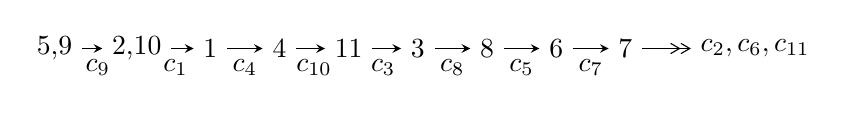
\begin{tikzpicture}[x=25pt, y=7pt]
	% node
	\node (A0) at (-1/8, 0) {5,9};
	\node (A1) at (17/16, 0) {2,10};
	\node (A2) at (17/8, 0) {1};
	\node (A3) at (25/8, 0) {4};
	\node (A4) at (33/8, 0) {11};
	\node (A5) at (41/8, 0) {3};
	\node (A6) at (49/8, 0) {8};
	\node (A7) at (57/8, 0) {6};
	\node (A8) at (65/8, 0) {7};
	\node (C1) at (1/2, -1) {$c_{9}$};
	\node (C2) at (13/8, -1) {$c_{1}$};
	\node (C3) at (21/8, -1) {$c_{4}$};
	\node (C4) at (29/8, -1) {$c_{10}$};
	\node (C5) at (37/8, -1) {$c_{3}$};
	\node (C6) at (45/8, -1) {$c_{8}$};
	\node (C7) at (53/8, -1) {$c_{5}$};
	\node (C8) at (61/8, -1) {$c_{7}$};
	\node (A9) at (10, 0) {$c_{2},c_{6},c_{11}$};

	% edge
	\draw[->,>=stealth]	
	(A0) edge (A1) (A1) edge (A2) (A2) edge (A3) (A3) edge (A4) (A4) edge (A5) (A5) edge (A6) (A6) edge (A7) (A7) edge (A8) ;
	\draw[->>,>={angle 60}]	
	(A8) edge (A9);
\end{tikzpicture} \\ 

\end{tabular} \\

\footnotetext{
The image of knot diagram is generated by the software ``\textbf{Draw programme}" developed by Andrew Bartholomew(\url{http://www.layer8.co.uk/maths/draw/index.htm\#Running-draw}), where we modified some parts for our purpose(\url{https://github.com/CATsTAILs/LinksPainter}).
}\phantom \\ \newline 
\centering \textbf{Ideals for irreducible components\footnotemark of $X_{\text{par}}$} 
 
\begin{align*}
I^u_{1}&=\langle 
256000670808631 u^{21}+674760339816179 u^{20}+\cdots+232517605023576 b+5745913318570412,\\
\phantom{I^u_{1}}&\phantom{= \langle  }3.63354\times10^{15} u^{21}+9.67535\times10^{15} u^{20}+\cdots+1.86014\times10^{15} a+8.31691\times10^{16},\;u^{22}+3 u^{21}+\cdots+56 u+8\rangle \\
I^u_{2}&=\langle 
2 u^{17} a+2 u^{17}+\cdots+a+6,\;-10 u^{17} a+23 u^{17}+\cdots-19 a+63,\;u^{18}- u^{17}+\cdots+3 u-1\rangle \\
I^u_{3}&=\langle 
b-1,\;4 a- u+2,\;u^2+2\rangle \\
\\
I^v_{1}&=\langle 
a,\;b+1,\;2 v-1\rangle \\
\end{align*}
\raggedright * 4 irreducible components of $\dim_{\mathbb{C}}=0$, with total 61 representations.\\
\footnotetext{All coefficients of polynomials are rational numbers. But the coefficients are sometimes approximated in decimal forms when there is not enough margin.}
\newpage
\renewcommand{\arraystretch}{1}
\centering \section*{I. $I^u_{1}= \langle 2.56\times10^{14} u^{21}+6.75\times10^{14} u^{20}+\cdots+2.33\times10^{14} b+5.75\times10^{15},\;3.63\times10^{15} u^{21}+9.68\times10^{15} u^{20}+\cdots+1.86\times10^{15} a+8.32\times10^{16},\;u^{22}+3 u^{21}+\cdots+56 u+8 \rangle$}
\flushleft \textbf{(i) Arc colorings}\\
\begin{tabular}{m{7pt} m{180pt} m{7pt} m{180pt} }
\flushright $a_{5}=$&$\begin{pmatrix}0\\u\end{pmatrix}$ \\
\flushright $a_{9}=$&$\begin{pmatrix}1\\0\end{pmatrix}$ \\
\flushright $a_{2}=$&$\begin{pmatrix}-1.95337 u^{21}-5.20141 u^{20}+\cdots-184.686 u-44.7112\\-1.10099 u^{21}-2.90198 u^{20}+\cdots-104.609 u-24.7117\end{pmatrix}$ \\
\flushright $a_{10}=$&$\begin{pmatrix}1\\u^2\end{pmatrix}$ \\
\flushright $a_{1}=$&$\begin{pmatrix}-0.852375 u^{21}-2.29943 u^{20}+\cdots-80.0775 u-19.9995\\-1.10099 u^{21}-2.90198 u^{20}+\cdots-104.609 u-24.7117\end{pmatrix}$ \\
\flushright $a_{4}=$&$\begin{pmatrix}u\\u^3+u\end{pmatrix}$ \\
\flushright $a_{11}=$&$\begin{pmatrix}u^2+1\\u^4+2 u^2\end{pmatrix}$ \\
\flushright $a_{3}=$&$\begin{pmatrix}-0.410016 u^{21}-1.10389 u^{20}+\cdots-37.5475 u-9.64240\\-0.733210 u^{21}-1.92174 u^{20}+\cdots-68.1510 u-16.3230\end{pmatrix}$ \\
\flushright $a_{8}=$&$\begin{pmatrix}-0.193796 u^{21}-0.498389 u^{20}+\cdots-16.9193 u-2.65074\\-1.07925 u^{21}-2.88821 u^{20}+\cdots-100.094 u-23.3142\end{pmatrix}$ \\
\flushright $a_{6}=$&$\begin{pmatrix}-0.293649 u^{21}-0.752180 u^{20}+\cdots-26.8185 u-5.67130\\-0.746302 u^{21}-1.99347 u^{20}+\cdots-69.2277 u-16.3438\end{pmatrix}$ \\
\flushright $a_{7}=$&$\begin{pmatrix}1.06840 u^{21}+2.85509 u^{20}+\cdots+101.338 u+25.2691\\-0.787989 u^{21}-2.09142 u^{20}+\cdots-72.2901 u-16.6414\end{pmatrix}$\\ \flushright $a_{7}=$&$\begin{pmatrix}1.06840 u^{21}+2.85509 u^{20}+\cdots+101.338 u+25.2691\\-0.787989 u^{21}-2.09142 u^{20}+\cdots-72.2901 u-16.6414\end{pmatrix}$\\&\end{tabular}
\flushleft \textbf{(ii) Obstruction class $= -1$}\\~\\
\flushleft \textbf{(iii) Cusp Shapes $= \frac{1537891371251021}{310023473364768} u^{21}+\frac{3975035432412625}{310023473364768} u^{20}+\cdots+\frac{461879710488329}{1099374019024} u+\frac{7058304318144475}{77505868341192}$}\\~\\
\newpage\renewcommand{\arraystretch}{1}
\flushleft \textbf{(iv) u-Polynomials at the component}\newline \\
\begin{tabular}{m{50pt}|m{274pt}}
Crossings & \hspace{64pt}u-Polynomials at each crossing \\
\hline $$\begin{aligned}c_{1},c_{7},c_{8}\\c_{11}\end{aligned}$$&$\begin{aligned}
&u^{22}+u^{21}+\cdots-7 u-3
\end{aligned}$\\
\hline $$\begin{aligned}c_{2},c_{6}\end{aligned}$$&$\begin{aligned}
&u^{22}-9 u^{20}+\cdots+7 u-24
\end{aligned}$\\
\hline $$\begin{aligned}c_{3},c_{5}\end{aligned}$$&$\begin{aligned}
&8(8 u^{22}-20 u^{21}+\cdots-2 u^2+1)
\end{aligned}$\\
\hline $$\begin{aligned}c_{4},c_{9},c_{10}\end{aligned}$$&$\begin{aligned}
&u^{22}+3 u^{21}+\cdots+56 u+8
\end{aligned}$\\
\hline
\end{tabular}\\~\\
\newpage\renewcommand{\arraystretch}{1}
\flushleft \textbf{(v) Riley Polynomials at the component}\newline \\
\begin{tabular}{m{50pt}|m{274pt}}
Crossings & \hspace{64pt}Riley Polynomials at each crossing \\
\hline $$\begin{aligned}c_{1},c_{7},c_{8}\\c_{11}\end{aligned}$$&$\begin{aligned}
&y^{22}+9 y^{21}+\cdots-55 y+9
\end{aligned}$\\
\hline $$\begin{aligned}c_{2},c_{6}\end{aligned}$$&$\begin{aligned}
&y^{22}-18 y^{21}+\cdots+335 y+576
\end{aligned}$\\
\hline $$\begin{aligned}c_{3},c_{5}\end{aligned}$$&$\begin{aligned}
&64(64 y^{22}-240 y^{21}+\cdots-4 y+1)
\end{aligned}$\\
\hline $$\begin{aligned}c_{4},c_{9},c_{10}\end{aligned}$$&$\begin{aligned}
&y^{22}+21 y^{21}+\cdots-480 y+64
\end{aligned}$\\
\hline
\end{tabular}\\~\\
\newpage\flushleft \textbf{(vi) Complex Volumes and Cusp Shapes}
$$\begin{array}{c|c|c}  
\text{Solutions to }I^u_{1}& \I (\text{vol} + \sqrt{-1}CS) & \text{Cusp shape}\\
 \hline 
\begin{aligned}
u &= -0.923083 + 0.449241 I \\
a &= \phantom{-}0.46489 - 1.80679 I \\
b &= -0.471805 - 1.329800 I\end{aligned}
 & -9.5532 + 10.8949 I & -8.89518 - 7.36414 I \\ \hline\begin{aligned}
u &= -0.923083 - 0.449241 I \\
a &= \phantom{-}0.46489 + 1.80679 I \\
b &= -0.471805 + 1.329800 I\end{aligned}
 & -9.5532 - 10.8949 I & -8.89518 + 7.36414 I \\ \hline\begin{aligned}
u &= \phantom{-}1.051430 + 0.225174 I \\
a &= \phantom{-}0.06569 + 1.67599 I \\
b &= -0.304231 + 1.040140 I\end{aligned}
 & -3.20816 - 4.89414 I & -6.47528 + 9.10540 I \\ \hline\begin{aligned}
u &= \phantom{-}1.051430 - 0.225174 I \\
a &= \phantom{-}0.06569 - 1.67599 I \\
b &= -0.304231 - 1.040140 I\end{aligned}
 & -3.20816 + 4.89414 I & -6.47528 - 9.10540 I \\ \hline\begin{aligned}
u &= -0.879824 + 0.816752 I \\
a &= \phantom{-}0.559661 - 1.087650 I \\
b &= \phantom{-}0.313637 - 1.227100 I\end{aligned}
 & -8.56742 - 4.93041 I & -9.24363 + 4.50732 I \\ \hline\begin{aligned}
u &= -0.879824 - 0.816752 I \\
a &= \phantom{-}0.559661 + 1.087650 I \\
b &= \phantom{-}0.313637 + 1.227100 I\end{aligned}
 & -8.56742 + 4.93041 I & -9.24363 - 4.50732 I \\ \hline\begin{aligned}
u &= -0.123835 + 1.345220 I \\
a &= \phantom{-}0.527565 - 0.232201 I \\
b &= -1.43217 + 0.42237 I\end{aligned}
 & \phantom{-}4.03174 + 1.74144 I & -4.49330 - 4.13639 I \\ \hline\begin{aligned}
u &= -0.123835 - 1.345220 I \\
a &= \phantom{-}0.527565 + 0.232201 I \\
b &= -1.43217 - 0.42237 I\end{aligned}
 & \phantom{-}4.03174 - 1.74144 I & -4.49330 + 4.13639 I \\ \hline\begin{aligned}
u &= -0.613996 + 1.252680 I \\
a &= -0.426413 + 1.140360 I \\
b &= \phantom{-}0.267923 + 0.935360 I\end{aligned}
 & \phantom{-}0.17781 + 3.00927 I & -2.42568 - 8.45199 I \\ \hline\begin{aligned}
u &= -0.613996 - 1.252680 I \\
a &= -0.426413 - 1.140360 I \\
b &= \phantom{-}0.267923 - 0.935360 I\end{aligned}
 & \phantom{-}0.17781 - 3.00927 I & -2.42568 + 8.45199 I\\
 \hline 
 \end{array}$$\newpage$$\begin{array}{c|c|c}  
\text{Solutions to }I^u_{1}& \I (\text{vol} + \sqrt{-1}CS) & \text{Cusp shape}\\
 \hline 
\begin{aligned}
u &= \phantom{-}0.051311 + 0.543007 I \\
a &= \phantom{-}0.085673 + 0.510275 I \\
b &= \phantom{-}0.531392 + 0.374501 I\end{aligned}
 & \phantom{-}0.81916 + 1.15831 I & \phantom{-}3.24306 - 4.91464 I \\ \hline\begin{aligned}
u &= \phantom{-}0.051311 - 0.543007 I \\
a &= \phantom{-}0.085673 - 0.510275 I \\
b &= \phantom{-}0.531392 - 0.374501 I\end{aligned}
 & \phantom{-}0.81916 - 1.15831 I & \phantom{-}3.24306 + 4.91464 I \\ \hline\begin{aligned}
u &= \phantom{-}0.07053 + 1.46071 I \\
a &= \phantom{-}0.392040 + 0.012145 I \\
b &= -0.893893 - 0.461606 I\end{aligned}
 & \phantom{-}7.21746 + 0.43098 I & \phantom{-}4.81736 - 2.08890 I \\ \hline\begin{aligned}
u &= \phantom{-}0.07053 - 1.46071 I \\
a &= \phantom{-}0.392040 - 0.012145 I \\
b &= -0.893893 + 0.461606 I\end{aligned}
 & \phantom{-}7.21746 - 0.43098 I & \phantom{-}4.81736 + 2.08890 I \\ \hline\begin{aligned}
u &= \phantom{-}0.38554 + 1.45702 I \\
a &= -0.858101 - 1.123100 I \\
b &= \phantom{-}0.519928 - 1.174350 I\end{aligned}
 & \phantom{-}2.25077 - 9.90431 I & -2.68871 + 7.61704 I \\ \hline\begin{aligned}
u &= \phantom{-}0.38554 - 1.45702 I \\
a &= -0.858101 + 1.123100 I \\
b &= \phantom{-}0.519928 + 1.174350 I\end{aligned}
 & \phantom{-}2.25077 + 9.90431 I & -2.68871 - 7.61704 I \\ \hline\begin{aligned}
u &= -0.34668 + 1.51369 I \\
a &= -1.07441 + 0.97292 I \\
b &= \phantom{-}0.60863 + 1.34961 I\end{aligned}
 & -3.2485 + 15.4927 I & -5.17708 - 7.97844 I \\ \hline\begin{aligned}
u &= -0.34668 - 1.51369 I \\
a &= -1.07441 - 0.97292 I \\
b &= \phantom{-}0.60863 - 1.34961 I\end{aligned}
 & -3.2485 - 15.4927 I & -5.17708 + 7.97844 I \\ \hline\begin{aligned}
u &= -0.364239\phantom{ +0.000000I} \\
a &= \phantom{-}0.703521\phantom{ +0.000000I} \\
b &= \phantom{-}1.25729\phantom{ +0.000000I}\end{aligned}
 & -0.360724\phantom{ +0.000000I} & -18.5120\phantom{ +0.000000I} \\ \hline\begin{aligned}
u &= -0.342457\phantom{ +0.000000I} \\
a &= -1.98069\phantom{ +0.000000I} \\
b &= -0.295995\phantom{ +0.000000I}\end{aligned}
 & -1.11076\phantom{ +0.000000I} & -11.5720\phantom{ +0.000000I}\\
 \hline 
 \end{array}$$\newpage$$\begin{array}{c|c|c}  
\text{Solutions to }I^u_{1}& \I (\text{vol} + \sqrt{-1}CS) & \text{Cusp shape}\\
 \hline 
\begin{aligned}
u &= \phantom{-}0.18195 + 1.70803 I \\
a &= \phantom{-}0.276992 + 0.588080 I \\
b &= -0.120052 + 0.802501 I\end{aligned}
 & \phantom{-}1.76897 - 0.99297 I & \phantom{-}2.13017 + 4.98419 I \\ \hline\begin{aligned}
u &= \phantom{-}0.18195 - 1.70803 I \\
a &= \phantom{-}0.276992 - 0.588080 I \\
b &= -0.120052 - 0.802501 I\end{aligned}
 & \phantom{-}1.76897 + 0.99297 I & \phantom{-}2.13017 - 4.98419 I\\
 \hline 
 \end{array}$$\newpage\newpage\renewcommand{\arraystretch}{1}
\centering \section*{II. $I^u_{2}= \langle 2 u^{17} a+2 u^{17}+\cdots+a+6,\;-10 u^{17} a+23 u^{17}+\cdots-19 a+63,\;u^{18}- u^{17}+\cdots+3 u-1 \rangle$}
\flushleft \textbf{(i) Arc colorings}\\
\begin{tabular}{m{7pt} m{180pt} m{7pt} m{180pt} }
\flushright $a_{5}=$&$\begin{pmatrix}0\\u\end{pmatrix}$ \\
\flushright $a_{9}=$&$\begin{pmatrix}1\\0\end{pmatrix}$ \\
\flushright $a_{2}=$&$\begin{pmatrix}a\\-\frac{2}{5} u^{17} a-\frac{2}{5} u^{17}+\cdots-\frac{1}{5} a-\frac{6}{5}\end{pmatrix}$ \\
\flushright $a_{10}=$&$\begin{pmatrix}1\\u^2\end{pmatrix}$ \\
\flushright $a_{1}=$&$\begin{pmatrix}\frac{2}{5} u^{17} a+\frac{2}{5} u^{17}+\cdots+\frac{6}{5} a+\frac{6}{5}\\-\frac{2}{5} u^{17} a-\frac{2}{5} u^{17}+\cdots-\frac{1}{5} a-\frac{6}{5}\end{pmatrix}$ \\
\flushright $a_{4}=$&$\begin{pmatrix}u\\u^3+u\end{pmatrix}$ \\
\flushright $a_{11}=$&$\begin{pmatrix}u^2+1\\u^4+2 u^2\end{pmatrix}$ \\
\flushright $a_{3}=$&$\begin{pmatrix}1.06667 a u^{17}-1.26667 u^{17}+\cdots+1.86667 a-1.13333\\-0.200000 a u^{17}-1.53333 u^{17}+\cdots+0.400000 a-2.93333\end{pmatrix}$ \\
\flushright $a_{8}=$&$\begin{pmatrix}\frac{2}{5} u^{17} a-\frac{34}{15} u^{17}+\cdots+\frac{6}{5} a-\frac{82}{15}\\-\frac{2}{5} u^{17} a-\frac{2}{5} u^{17}+\cdots-\frac{1}{5} a-\frac{6}{5}\end{pmatrix}$ \\
\flushright $a_{6}=$&$\begin{pmatrix}1.53333 a u^{17}-1.46667 u^{17}+\cdots+2.93333 a-5.40000\\-0.400000 a u^{17}-1.06667 u^{17}+\cdots+0.800000 a-1.86667\end{pmatrix}$ \\
\flushright $a_{7}=$&$\begin{pmatrix}\frac{2}{5} u^{17} a-\frac{34}{15} u^{17}+\cdots+\frac{6}{5} a-\frac{97}{15}\\-1\end{pmatrix}$\\ \flushright $a_{7}=$&$\begin{pmatrix}\frac{2}{5} u^{17} a-\frac{34}{15} u^{17}+\cdots+\frac{6}{5} a-\frac{97}{15}\\-1\end{pmatrix}$\\&\end{tabular}
\flushleft \textbf{(ii) Obstruction class $= -1$}\\~\\
\flushleft \textbf{(iii) Cusp Shapes $= -4 u^{17}+4 u^{16}-36 u^{15}+28 u^{14}-124 u^{13}+72 u^{12}-196 u^{11}+72 u^{10}-120 u^9+8 u^7-36 u^6+8 u^5-4 u^4-16 u^3+8 u-14$}\\~\\
\newpage\renewcommand{\arraystretch}{1}
\flushleft \textbf{(iv) u-Polynomials at the component}\newline \\
\begin{tabular}{m{50pt}|m{274pt}}
Crossings & \hspace{64pt}u-Polynomials at each crossing \\
\hline $$\begin{aligned}c_{1},c_{7},c_{8}\\c_{11}\end{aligned}$$&$\begin{aligned}
&u^{36}-3 u^{35}+\cdots-8 u+1
\end{aligned}$\\
\hline $$\begin{aligned}c_{2},c_{6}\end{aligned}$$&$\begin{aligned}
&(u^{18}+u^{17}+\cdots- u-1)^{2}
\end{aligned}$\\
\hline $$\begin{aligned}c_{3},c_{5}\end{aligned}$$&$\begin{aligned}
&9(9 u^{36}+27 u^{35}+\cdots-20172 u+3559)
\end{aligned}$\\
\hline $$\begin{aligned}c_{4},c_{9},c_{10}\end{aligned}$$&$\begin{aligned}
&(u^{18}- u^{17}+\cdots+3 u-1)^{2}
\end{aligned}$\\
\hline
\end{tabular}\\~\\
\newpage\renewcommand{\arraystretch}{1}
\flushleft \textbf{(v) Riley Polynomials at the component}\newline \\
\begin{tabular}{m{50pt}|m{274pt}}
Crossings & \hspace{64pt}Riley Polynomials at each crossing \\
\hline $$\begin{aligned}c_{1},c_{7},c_{8}\\c_{11}\end{aligned}$$&$\begin{aligned}
&y^{36}+23 y^{35}+\cdots-16 y+1
\end{aligned}$\\
\hline $$\begin{aligned}c_{2},c_{6}\end{aligned}$$&$\begin{aligned}
&(y^{18}-15 y^{17}+\cdots-7 y+1)^{2}
\end{aligned}$\\
\hline $$\begin{aligned}c_{3},c_{5}\end{aligned}$$&$\begin{aligned}
&81(81 y^{36}-1377 y^{35}+\cdots-7.10112\times10^{7} y+1.26665\times10^{7})
\end{aligned}$\\
\hline $$\begin{aligned}c_{4},c_{9},c_{10}\end{aligned}$$&$\begin{aligned}
&(y^{18}+17 y^{17}+\cdots-7 y+1)^{2}
\end{aligned}$\\
\hline
\end{tabular}\\~\\
\newpage\flushleft \textbf{(vi) Complex Volumes and Cusp Shapes}
$$\begin{array}{c|c|c}  
\text{Solutions to }I^u_{2}& \I (\text{vol} + \sqrt{-1}CS) & \text{Cusp shape}\\
 \hline 
\begin{aligned}
u &= -0.215059 + 1.214380 I \\
a &= -1.264270 + 0.313519 I \\
b &= \phantom{-}0.816163 + 1.122800 I\end{aligned}
 & -5.44315 + 3.22673 I & -7.05526 - 3.62956 I \\ \hline\begin{aligned}
u &= -0.215059 + 1.214380 I \\
a &= \phantom{-}0.121854 - 0.436704 I \\
b &= \phantom{-}0.27308 - 1.57039 I\end{aligned}
 & -5.44315 + 3.22673 I & -7.05526 - 3.62956 I \\ \hline\begin{aligned}
u &= -0.215059 - 1.214380 I \\
a &= -1.264270 - 0.313519 I \\
b &= \phantom{-}0.816163 - 1.122800 I\end{aligned}
 & -5.44315 - 3.22673 I & -7.05526 + 3.62956 I \\ \hline\begin{aligned}
u &= -0.215059 - 1.214380 I \\
a &= \phantom{-}0.121854 + 0.436704 I \\
b &= \phantom{-}0.27308 + 1.57039 I\end{aligned}
 & -5.44315 - 3.22673 I & -7.05526 + 3.62956 I \\ \hline\begin{aligned}
u &= \phantom{-}0.678984 + 0.355286 I \\
a &= -0.359076 + 0.145322 I \\
b &= -1.008890 + 0.077944 I\end{aligned}
 & -5.17867 - 5.71427 I & -7.06596 + 6.05983 I \\ \hline\begin{aligned}
u &= \phantom{-}0.678984 + 0.355286 I \\
a &= -0.41568 - 1.94193 I \\
b &= \phantom{-}0.46000 - 1.36593 I\end{aligned}
 & -5.17867 - 5.71427 I & -7.06596 + 6.05983 I \\ \hline\begin{aligned}
u &= \phantom{-}0.678984 - 0.355286 I \\
a &= -0.359076 - 0.145322 I \\
b &= -1.008890 - 0.077944 I\end{aligned}
 & -5.17867 + 5.71427 I & -7.06596 - 6.05983 I \\ \hline\begin{aligned}
u &= \phantom{-}0.678984 - 0.355286 I \\
a &= -0.41568 + 1.94193 I \\
b &= \phantom{-}0.46000 + 1.36593 I\end{aligned}
 & -5.17867 + 5.71427 I & -7.06596 - 6.05983 I \\ \hline\begin{aligned}
u &= -0.590027 + 0.406016 I \\
a &= -0.254655 + 0.532993 I \\
b &= -0.430436 + 0.146579 I\end{aligned}
 & -0.86368 + 1.88569 I & -1.68331 - 3.99357 I \\ \hline\begin{aligned}
u &= -0.590027 + 0.406016 I \\
a &= -0.66911 + 1.67095 I \\
b &= \phantom{-}0.259835 + 0.987292 I\end{aligned}
 & -0.86368 + 1.88569 I & -1.68331 - 3.99357 I\\
 \hline 
 \end{array}$$\newpage$$\begin{array}{c|c|c}  
\text{Solutions to }I^u_{2}& \I (\text{vol} + \sqrt{-1}CS) & \text{Cusp shape}\\
 \hline 
\begin{aligned}
u &= -0.590027 - 0.406016 I \\
a &= -0.254655 - 0.532993 I \\
b &= -0.430436 - 0.146579 I\end{aligned}
 & -0.86368 - 1.88569 I & -1.68331 + 3.99357 I \\ \hline\begin{aligned}
u &= -0.590027 - 0.406016 I \\
a &= -0.66911 - 1.67095 I \\
b &= \phantom{-}0.259835 - 0.987292 I\end{aligned}
 & -0.86368 - 1.88569 I & -1.68331 + 3.99357 I \\ \hline\begin{aligned}
u &= \phantom{-}0.482433 + 0.528989 I \\
a &= -0.01159 - 1.42789 I \\
b &= \phantom{-}0.535422 + 0.229537 I\end{aligned}
 & -4.41864 + 1.78695 I & -5.23943 + 0.02251 I \\ \hline\begin{aligned}
u &= \phantom{-}0.482433 + 0.528989 I \\
a &= -1.59986 - 0.89994 I \\
b &= -0.182954 - 1.202280 I\end{aligned}
 & -4.41864 + 1.78695 I & -5.23943 + 0.02251 I \\ \hline\begin{aligned}
u &= \phantom{-}0.482433 - 0.528989 I \\
a &= -0.01159 + 1.42789 I \\
b &= \phantom{-}0.535422 - 0.229537 I\end{aligned}
 & -4.41864 - 1.78695 I & -5.23943 - 0.02251 I \\ \hline\begin{aligned}
u &= \phantom{-}0.482433 - 0.528989 I \\
a &= -1.59986 + 0.89994 I \\
b &= -0.182954 + 1.202280 I\end{aligned}
 & -4.41864 - 1.78695 I & -5.23943 - 0.02251 I \\ \hline\begin{aligned}
u &= \phantom{-}0.076050 + 1.298790 I \\
a &= -0.36644 + 1.56815 I \\
b &= \phantom{-}0.181838 + 1.232260 I\end{aligned}
 & \phantom{-}0.06375 - 1.57187 I & -1.80878 + 4.22070 I \\ \hline\begin{aligned}
u &= \phantom{-}0.076050 + 1.298790 I \\
a &= -1.80534 - 0.43101 I \\
b &= \phantom{-}0.393324 - 0.963175 I\end{aligned}
 & \phantom{-}0.06375 - 1.57187 I & -1.80878 + 4.22070 I \\ \hline\begin{aligned}
u &= \phantom{-}0.076050 - 1.298790 I \\
a &= -0.36644 - 1.56815 I \\
b &= \phantom{-}0.181838 - 1.232260 I\end{aligned}
 & \phantom{-}0.06375 + 1.57187 I & -1.80878 - 4.22070 I \\ \hline\begin{aligned}
u &= \phantom{-}0.076050 - 1.298790 I \\
a &= -1.80534 + 0.43101 I \\
b &= \phantom{-}0.393324 + 0.963175 I\end{aligned}
 & \phantom{-}0.06375 + 1.57187 I & -1.80878 - 4.22070 I\\
 \hline 
 \end{array}$$\newpage$$\begin{array}{c|c|c}  
\text{Solutions to }I^u_{2}& \I (\text{vol} + \sqrt{-1}CS) & \text{Cusp shape}\\
 \hline 
\begin{aligned}
u &= -0.663049\phantom{ +0.000000I} \\
a &= \phantom{-}0.21254 + 1.83196 I \\
b &= -0.53627 + 1.36483 I\end{aligned}
 & -9.12242\phantom{ +0.000000I} & -12.3720\phantom{ +0.000000I} \\ \hline\begin{aligned}
u &= -0.663049\phantom{ +0.000000I} \\
a &= \phantom{-}0.21254 - 1.83196 I \\
b &= -0.53627 - 1.36483 I\end{aligned}
 & -9.12242\phantom{ +0.000000I} & -12.3720\phantom{ +0.000000I} \\ \hline\begin{aligned}
u &= \phantom{-}0.17132 + 1.45278 I \\
a &= \phantom{-}0.948480 + 0.683751 I \\
b &= -0.119141 + 0.939188 I\end{aligned}
 & \phantom{-}1.85527 - 0.55896 I & -1.51114 - 0.25710 I \\ \hline\begin{aligned}
u &= \phantom{-}0.17132 + 1.45278 I \\
a &= -0.002433 + 0.666631 I \\
b &= \phantom{-}0.197872 + 0.137215 I\end{aligned}
 & \phantom{-}1.85527 - 0.55896 I & -1.51114 - 0.25710 I \\ \hline\begin{aligned}
u &= \phantom{-}0.17132 - 1.45278 I \\
a &= \phantom{-}0.948480 - 0.683751 I \\
b &= -0.119141 - 0.939188 I\end{aligned}
 & \phantom{-}1.85527 + 0.55896 I & -1.51114 + 0.25710 I \\ \hline\begin{aligned}
u &= \phantom{-}0.17132 - 1.45278 I \\
a &= -0.002433 - 0.666631 I \\
b &= \phantom{-}0.197872 - 0.137215 I\end{aligned}
 & \phantom{-}1.85527 + 0.55896 I & -1.51114 + 0.25710 I \\ \hline\begin{aligned}
u &= \phantom{-}0.25789 + 1.44398 I \\
a &= \phantom{-}0.995814 + 0.788845 I \\
b &= -0.69402 + 1.37640 I\end{aligned}
 & \phantom{-}0.60037 - 9.13509 I & -2.98695 + 5.86478 I \\ \hline\begin{aligned}
u &= \phantom{-}0.25789 + 1.44398 I \\
a &= -0.379824 - 0.352640 I \\
b &= \phantom{-}1.211220 + 0.140810 I\end{aligned}
 & \phantom{-}0.60037 - 9.13509 I & -2.98695 + 5.86478 I \\ \hline\begin{aligned}
u &= \phantom{-}0.25789 - 1.44398 I \\
a &= \phantom{-}0.995814 - 0.788845 I \\
b &= -0.69402 - 1.37640 I\end{aligned}
 & \phantom{-}0.60037 + 9.13509 I & -2.98695 - 5.86478 I \\ \hline\begin{aligned}
u &= \phantom{-}0.25789 - 1.44398 I \\
a &= -0.379824 + 0.352640 I \\
b &= \phantom{-}1.211220 - 0.140810 I\end{aligned}
 & \phantom{-}0.60037 + 9.13509 I & -2.98695 - 5.86478 I\\
 \hline 
 \end{array}$$\newpage$$\begin{array}{c|c|c}  
\text{Solutions to }I^u_{2}& \I (\text{vol} + \sqrt{-1}CS) & \text{Cusp shape}\\
 \hline 
\begin{aligned}
u &= -0.22144 + 1.45044 I \\
a &= \phantom{-}0.938644 - 0.851386 I \\
b &= -0.554814 - 1.110360 I\end{aligned}
 & \phantom{-}5.09742 + 4.87394 I & \phantom{-}1.52680 - 3.60136 I \\ \hline\begin{aligned}
u &= -0.22144 + 1.45044 I \\
a &= -0.195603 + 0.086886 I \\
b &= \phantom{-}0.855022 - 0.244718 I\end{aligned}
 & \phantom{-}5.09742 + 4.87394 I & \phantom{-}1.52680 - 3.60136 I \\ \hline\begin{aligned}
u &= -0.22144 - 1.45044 I \\
a &= \phantom{-}0.938644 + 0.851386 I \\
b &= -0.554814 + 1.110360 I\end{aligned}
 & \phantom{-}5.09742 - 4.87394 I & \phantom{-}1.52680 + 3.60136 I \\ \hline\begin{aligned}
u &= -0.22144 - 1.45044 I \\
a &= -0.195603 - 0.086886 I \\
b &= \phantom{-}0.855022 + 0.244718 I\end{aligned}
 & \phantom{-}5.09742 - 4.87394 I & \phantom{-}1.52680 + 3.60136 I \\ \hline\begin{aligned}
u &= \phantom{-}0.382766\phantom{ +0.000000I} \\
a &= \phantom{-}2.60655 + 3.77847 I \\
b &= -0.157243 + 1.036420 I\end{aligned}
 & -3.91179\phantom{ +0.000000I} & -11.9800\phantom{ +0.000000I} \\ \hline\begin{aligned}
u &= \phantom{-}0.382766\phantom{ +0.000000I} \\
a &= \phantom{-}2.60655 - 3.77847 I \\
b &= -0.157243 - 1.036420 I\end{aligned}
 & -3.91179\phantom{ +0.000000I} & -11.9800\phantom{ +0.000000I}\\
 \hline 
 \end{array}$$\newpage\newpage\renewcommand{\arraystretch}{1}
\centering \section*{III. $I^u_{3}= \langle b-1,\;4 a- u+2,\;u^2+2 \rangle$}
\flushleft \textbf{(i) Arc colorings}\\
\begin{tabular}{m{7pt} m{180pt} m{7pt} m{180pt} }
\flushright $a_{5}=$&$\begin{pmatrix}0\\u\end{pmatrix}$ \\
\flushright $a_{9}=$&$\begin{pmatrix}1\\0\end{pmatrix}$ \\
\flushright $a_{2}=$&$\begin{pmatrix}\frac{1}{4} u-\frac{1}{2}\\1\end{pmatrix}$ \\
\flushright $a_{10}=$&$\begin{pmatrix}1\\-2\end{pmatrix}$ \\
\flushright $a_{1}=$&$\begin{pmatrix}\frac{1}{4} u-\frac{3}{2}\\1\end{pmatrix}$ \\
\flushright $a_{4}=$&$\begin{pmatrix}u\\- u\end{pmatrix}$ \\
\flushright $a_{11}=$&$\begin{pmatrix}-1\\0\end{pmatrix}$ \\
\flushright $a_{3}=$&$\begin{pmatrix}\frac{3}{8} u-1\\-\frac{1}{2} u+\frac{1}{2}\end{pmatrix}$ \\
\flushright $a_{8}=$&$\begin{pmatrix}\frac{1}{4} u+\frac{1}{2}\\1\end{pmatrix}$ \\
\flushright $a_{6}=$&$\begin{pmatrix}-\frac{1}{8} u+\frac{1}{2}\\\frac{1}{2} u+\frac{1}{2}\end{pmatrix}$ \\
\flushright $a_{7}=$&$\begin{pmatrix}\frac{1}{4} u-\frac{1}{2}\\1\end{pmatrix}$\\ \flushright $a_{7}=$&$\begin{pmatrix}\frac{1}{4} u-\frac{1}{2}\\1\end{pmatrix}$\\&\end{tabular}
\flushleft \textbf{(ii) Obstruction class $= 1$}\\~\\
\flushleft \textbf{(iii) Cusp Shapes $= 0$}\\~\\
\newpage\renewcommand{\arraystretch}{1}
\flushleft \textbf{(iv) u-Polynomials at the component}\newline \\
\begin{tabular}{m{50pt}|m{274pt}}
Crossings & \hspace{64pt}u-Polynomials at each crossing \\
\hline $$\begin{aligned}c_{1},c_{2},c_{11}\end{aligned}$$&$\begin{aligned}
&(u+1)^2
\end{aligned}$\\
\hline $$\begin{aligned}c_{3}\end{aligned}$$&$\begin{aligned}
&4(4 u^2+4 u+3)
\end{aligned}$\\
\hline $$\begin{aligned}c_{4},c_{9},c_{10}\end{aligned}$$&$\begin{aligned}
&u^2+2
\end{aligned}$\\
\hline $$\begin{aligned}c_{5}\end{aligned}$$&$\begin{aligned}
&4(4 u^2-4 u+3)
\end{aligned}$\\
\hline $$\begin{aligned}c_{6},c_{7},c_{8}\end{aligned}$$&$\begin{aligned}
&(u-1)^2
\end{aligned}$\\
\hline
\end{tabular}\\~\\
\newpage\renewcommand{\arraystretch}{1}
\flushleft \textbf{(v) Riley Polynomials at the component}\newline \\
\begin{tabular}{m{50pt}|m{274pt}}
Crossings & \hspace{64pt}Riley Polynomials at each crossing \\
\hline $$\begin{aligned}c_{1},c_{2},c_{6}\\c_{7},c_{8},c_{11}\end{aligned}$$&$\begin{aligned}
&(y-1)^2
\end{aligned}$\\
\hline $$\begin{aligned}c_{3},c_{5}\end{aligned}$$&$\begin{aligned}
&16(16 y^2+8 y+9)
\end{aligned}$\\
\hline $$\begin{aligned}c_{4},c_{9},c_{10}\end{aligned}$$&$\begin{aligned}
&(y+2)^2
\end{aligned}$\\
\hline
\end{tabular}\\~\\
\newpage\flushleft \textbf{(vi) Complex Volumes and Cusp Shapes}
$$\begin{array}{c|c|c}  
\text{Solutions to }I^u_{3}& \I (\text{vol} + \sqrt{-1}CS) & \text{Cusp shape}\\
 \hline 
\begin{aligned}
u &= \phantom{-0.000000 -}1.414210 I \\
a &= -0.500000 + 0.353553 I \\
b &= \phantom{-}1.00000\phantom{ +0.000000I}\end{aligned}
 & \phantom{-}4.93480\phantom{ +0.000000I} & \phantom{-0.000000 } 0 \\ \hline\begin{aligned}
u &= \phantom{-0.000000 } -1.414210 I \\
a &= -0.500000 - 0.353553 I \\
b &= \phantom{-}1.00000\phantom{ +0.000000I}\end{aligned}
 & \phantom{-}4.93480\phantom{ +0.000000I} & \phantom{-0.000000 } 0\\
 \hline 
 \end{array}$$\newpage\newpage\renewcommand{\arraystretch}{1}
\centering \section*{IV. $I^v_{1}= \langle a,\;b+1,\;2 v-1 \rangle$}
\flushleft \textbf{(i) Arc colorings}\\
\begin{tabular}{m{7pt} m{180pt} m{7pt} m{180pt} }
\flushright $a_{5}=$&$\begin{pmatrix}0.5\\0\end{pmatrix}$ \\
\flushright $a_{9}=$&$\begin{pmatrix}1\\0\end{pmatrix}$ \\
\flushright $a_{2}=$&$\begin{pmatrix}0\\-1\end{pmatrix}$ \\
\flushright $a_{10}=$&$\begin{pmatrix}1\\0\end{pmatrix}$ \\
\flushright $a_{1}=$&$\begin{pmatrix}1\\-1\end{pmatrix}$ \\
\flushright $a_{4}=$&$\begin{pmatrix}0.5\\0\end{pmatrix}$ \\
\flushright $a_{11}=$&$\begin{pmatrix}1\\0\end{pmatrix}$ \\
\flushright $a_{3}=$&$\begin{pmatrix}1\\-0.5\end{pmatrix}$ \\
\flushright $a_{8}=$&$\begin{pmatrix}1\\1\end{pmatrix}$ \\
\flushright $a_{6}=$&$\begin{pmatrix}1\\0.5\end{pmatrix}$ \\
\flushright $a_{7}=$&$\begin{pmatrix}0\\1\end{pmatrix}$\\ \flushright $a_{7}=$&$\begin{pmatrix}0\\1\end{pmatrix}$\\&\end{tabular}
\flushleft \textbf{(ii) Obstruction class $= 1$}\\~\\
\flushleft \textbf{(iii) Cusp Shapes $= 4.5$}\\~\\
\newpage\renewcommand{\arraystretch}{1}
\flushleft \textbf{(iv) u-Polynomials at the component}\newline \\
\begin{tabular}{m{50pt}|m{274pt}}
Crossings & \hspace{64pt}u-Polynomials at each crossing \\
\hline $$\begin{aligned}c_{1},c_{2},c_{11}\end{aligned}$$&$\begin{aligned}
&u-1
\end{aligned}$\\
\hline $$\begin{aligned}c_{3}\end{aligned}$$&$\begin{aligned}
&2(2 u+1)
\end{aligned}$\\
\hline $$\begin{aligned}c_{4},c_{9},c_{10}\end{aligned}$$&$\begin{aligned}
&u
\end{aligned}$\\
\hline $$\begin{aligned}c_{5}\end{aligned}$$&$\begin{aligned}
&2(2 u-1)
\end{aligned}$\\
\hline $$\begin{aligned}c_{6},c_{7},c_{8}\end{aligned}$$&$\begin{aligned}
&u+1
\end{aligned}$\\
\hline
\end{tabular}\\~\\
\newpage\renewcommand{\arraystretch}{1}
\flushleft \textbf{(v) Riley Polynomials at the component}\newline \\
\begin{tabular}{m{50pt}|m{274pt}}
Crossings & \hspace{64pt}Riley Polynomials at each crossing \\
\hline $$\begin{aligned}c_{1},c_{2},c_{6}\\c_{7},c_{8},c_{11}\end{aligned}$$&$\begin{aligned}
&y-1
\end{aligned}$\\
\hline $$\begin{aligned}c_{3},c_{5}\end{aligned}$$&$\begin{aligned}
&4(4 y-1)
\end{aligned}$\\
\hline $$\begin{aligned}c_{4},c_{9},c_{10}\end{aligned}$$&$\begin{aligned}
&y
\end{aligned}$\\
\hline
\end{tabular}\\~\\
\newpage\flushleft \textbf{(vi) Complex Volumes and Cusp Shapes}
$$\begin{array}{c|c|c}  
\text{Solutions to }I^v_{1}& \I (\text{vol} + \sqrt{-1}CS) & \text{Cusp shape}\\
 \hline 
\begin{aligned}
v &= \phantom{-}0.500000\phantom{ +0.000000I} \\
a &= \phantom{-0.000000 } 0 \\
b &= -1.00000\phantom{ +0.000000I}\end{aligned}
 & \phantom{-0.000000 } 0 & \phantom{-}4.50000\phantom{ +0.000000I}\\
 \hline 
 \end{array}$$\newpage
\newpage\renewcommand{\arraystretch}{1}
\centering \section*{ V. u-Polynomials}
\begin{tabular}{m{50pt}|m{274pt}}
Crossings & \hspace{64pt}u-Polynomials at each crossing \\
\hline $$\begin{aligned}c_{1},c_{11}\end{aligned}$$&$\begin{aligned}
&(u-1)(u+1)^2(u^{22}+u^{21}+\cdots-7 u-3)(u^{36}-3 u^{35}+\cdots-8 u+1)
\end{aligned}$\\
\hline $$\begin{aligned}c_{2}\end{aligned}$$&$\begin{aligned}
&(u-1)(u+1)^2(u^{18}+u^{17}+\cdots- u-1)^{2}(u^{22}-9 u^{20}+\cdots+7 u-24)
\end{aligned}$\\
\hline $$\begin{aligned}c_{3}\end{aligned}$$&$\begin{aligned}
&576(2 u+1)(4 u^2+4 u+3)(8 u^{22}-20 u^{21}+\cdots-2 u^{2}+1)\\
&\cdot(9 u^{36}+27 u^{35}+\cdots-20172 u+3559)
\end{aligned}$\\
\hline $$\begin{aligned}c_{4},c_{9},c_{10}\end{aligned}$$&$\begin{aligned}
&u(u^2+2)(u^{18}- u^{17}+\cdots+3 u-1)^{2}(u^{22}+3 u^{21}+\cdots+56 u+8)
\end{aligned}$\\
\hline $$\begin{aligned}c_{5}\end{aligned}$$&$\begin{aligned}
&576(2 u-1)(4 u^2-4 u+3)(8 u^{22}-20 u^{21}+\cdots-2 u^{2}+1)\\
&\cdot(9 u^{36}+27 u^{35}+\cdots-20172 u+3559)
\end{aligned}$\\
\hline $$\begin{aligned}c_{6}\end{aligned}$$&$\begin{aligned}
&((u-1)^2)(u+1)(u^{18}+u^{17}+\cdots- u-1)^{2}(u^{22}-9 u^{20}+\cdots+7 u-24)
\end{aligned}$\\
\hline $$\begin{aligned}c_{7},c_{8}\end{aligned}$$&$\begin{aligned}
&((u-1)^2)(u+1)(u^{22}+u^{21}+\cdots-7 u-3)(u^{36}-3 u^{35}+\cdots-8 u+1)
\end{aligned}$\\
\hline
\end{tabular}\newpage\renewcommand{\arraystretch}{1}
\centering \section*{ VI. Riley Polynomials}
\begin{tabular}{m{50pt}|m{274pt}}
Crossings & \hspace{64pt}Riley Polynomials at each crossing \\
\hline $$\begin{aligned}c_{1},c_{7},c_{8}\\c_{11}\end{aligned}$$&$\begin{aligned}
&((y-1)^3)(y^{22}+9 y^{21}+\cdots-55 y+9)(y^{36}+23 y^{35}+\cdots-16 y+1)
\end{aligned}$\\
\hline $$\begin{aligned}c_{2},c_{6}\end{aligned}$$&$\begin{aligned}
&((y-1)^3)(y^{18}-15 y^{17}+\cdots-7 y+1)^{2}\\
&\cdot(y^{22}-18 y^{21}+\cdots+335 y+576)
\end{aligned}$\\
\hline $$\begin{aligned}c_{3},c_{5}\end{aligned}$$&$\begin{aligned}
&331776(4 y-1)(16 y^2+8 y+9)(64 y^{22}-240 y^{21}+\cdots-4 y+1)\\
&\cdot(81 y^{36}-1377 y^{35}+\cdots-71011164 y+12666481)
\end{aligned}$\\
\hline $$\begin{aligned}c_{4},c_{9},c_{10}\end{aligned}$$&$\begin{aligned}
&y(y+2)^2(y^{18}+17 y^{17}+\cdots-7 y+1)^{2}\\
&\cdot(y^{22}+21 y^{21}+\cdots-480 y+64)
\end{aligned}$\\
\hline
\end{tabular}
\vskip 2pc
\end{document}